\documentclass{bschlangaul-aufgabe}

\begin{document}
\bAufgabenMetadaten{
  Titel = {Aufgabe 2},
  Thematik = {Entwurfsmuster in UML-Diagramm erkennen},
  Referenz = 66116-2016-F.T1-TA2-A2,
  RelativerPfad = Staatsexamen/66116/2016/03/Thema-1/Teilaufgabe-2/Aufgabe-2.tex,
  ZitatSchluessel = examen:66116:2016:03,
  BearbeitungsStand = mit Lösung,
  Korrektheit = unbekannt,
  Ueberprueft = {unbekannt},
  Stichwoerter = {Klassendiagramm, Abstrakte Fabrik (Abstract Factory), Wiederholer (Iterator), Adapter, Kompositum (Composite), Klassenadapter, Objektadapter, Implementierung in Java},
  EinzelpruefungsNr = 66116,
  Jahr = 2016,
  Monat = 03,
  ThemaNr = 1,
  TeilaufgabeNr = 2,
  AufgabeNr = 2,
}

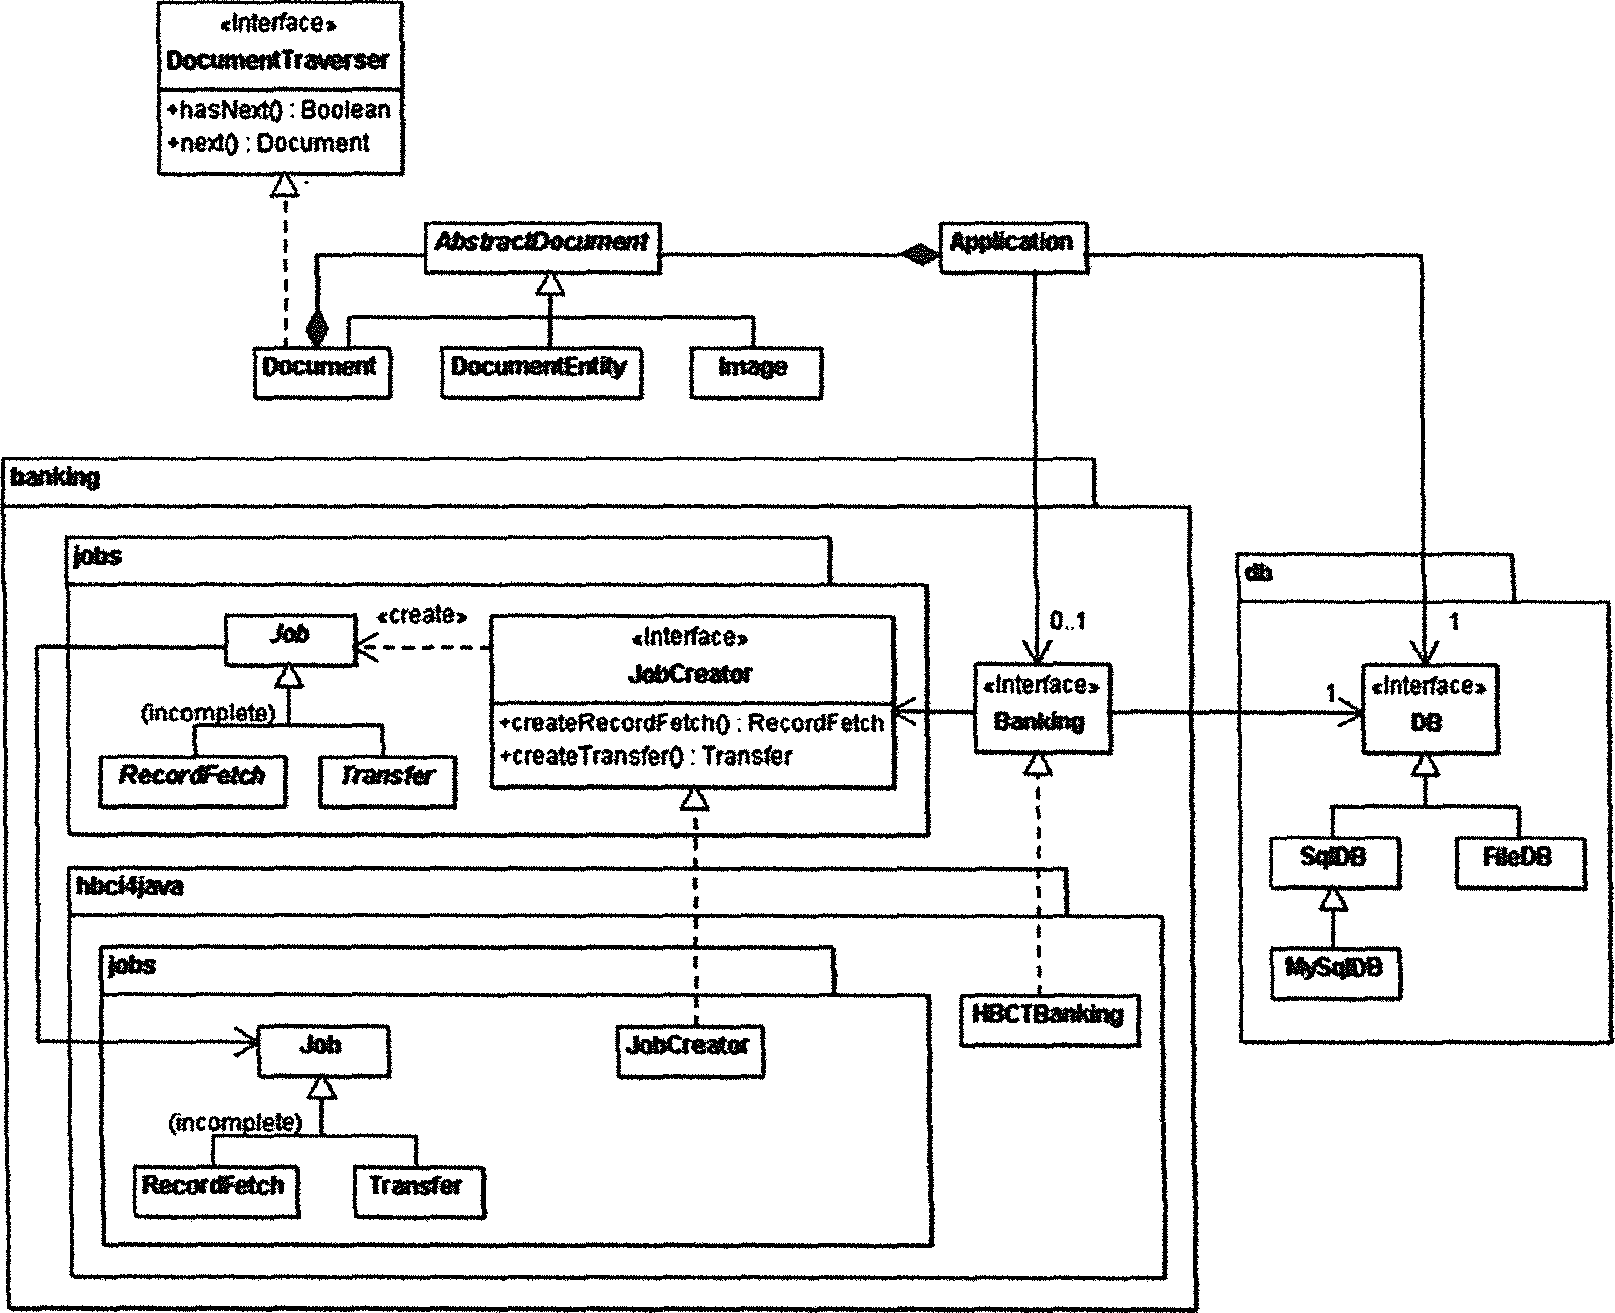
\includegraphics[width=\linewidth]{\bPfadAufgaben/Staatsexamen/66116/2016/03/Thema-1/Teilaufgabe-2/UML-Examen_2016-03.png}

\begin{enumerate}

%%
% 1.
%%

\item Kennzeichnen\footcite{examen:66116:2016:03} Sie im folgenden
Klassendiagramm\index{Klassendiagramm} die Entwurfsmuster
\emph{„Abstrakte Fabrik“}\index{Abstrakte Fabrik (Abstract Factory)},
\emph{„Iterator“}\index{Wiederholer (Iterator)}, \emph{„Adapter
“}\index{Adapter} und \emph{„Kompositum“}\index{Kompositum (Composite)}.
Geben Sie die jeweils beteiligten Klassen und deren Zuständigkeit im
entsprechenden Muster an.
\footcite{sosy:ab:6}

\begin{bAntwort}

\begin{description}

%%
%
%%

\item[Iterator] \strut

\begin{description}
\item[DocumentTraverser (interface)]
Schnittstelle zur Traversierung und zum Zugriff auf Dokumente

\item[Document]
implementiert die Schnittstelle
\end{description}

%%
%
%%

\item[Kompositum] \strut

\begin{description}
\item[AbstractDocument]
abstrakte Basisklasse, die gemeinsames Verhalten der beteiligten
Klassen definiert

\item[Document]
enthält wiederum weitere Documente bzw. DocumentEntities und Images

\item[DocumentEntity, Image]
primitive Unterklassen, besitzen keine Kindobjekte
\end{description}

%%
%
%%

\item[Adapter (Objektadapter)] \strut

\begin{description}
\item[Banking (interface)]
vom Client (hier Application) verwendete Schnittstelle

\item[HBCTBanking]
passt Schnittstelle der unpassenden Klasse an Zielschnittstelle
(Banking) an

\item[DB (interface)]
anzupassende Schnittstelle
\end{description}

%%
%
%%

\item[abstrakte Fabrik] \strut

\begin{description}
\item[JobCreator (interface)]
abstrakte Fabrik

\item[Job (abstrakt) mit Unterklassen RecordFetch und Transfer]
abstraktes Produkt

\item[Job (konkret) mit Unterklassen]
konkretes Produkt
\end{description}
\end{description}
\end{bAntwort}

%%
% 2.
%%

\item

\begin{enumerate}

%%
% (a)
%%

\item Beschreiben Sie die Funktionsweise der folgenden Entwurfsmuster
und geben Sie ein passendes UML-Diagramm an.

\begin{itemize}
\item Dekorierer
\item Klassenadapter
\item Objektadapter
\end{itemize}

\begin{bAntwort}
\bMetaNochKeineLoesung
\end{bAntwort}

%%
% (b)
%%

\item Erklären Sie mit maximal zwei Sätzen den Unterschied zwischen
Klassenadapter\index{Klassenadapter} und
Objektadapter\index{Objektadapter}.

\begin{bAntwort}
\bMetaNochKeineLoesung
\end{bAntwort}
\end{enumerate}

%%
% 3.
%%

\item Implementieren Sie einen Stapel in der Programmiersprache
Java.\index{Implementierung in Java} Nutzen Sie dazu ein Array mit
fester Größe. Auf eine Überlaufprüfung darf verzichtet werden.
Implementieren Sie in der Klasse das Iterator Entwurfsmuster, um auf die
Inhalte zuzugreifen, sowie eine Funktion zum Hinzufügen von Elementen.
Als Typ für den Stapel kann zur Vereinfachung ein Integertyp verwendet
werden.

\begin{bAntwort}
\bMetaNochKeineLoesung
\end{bAntwort}
\end{enumerate}
\end{document}
